\section{SoC Design Hardware}
\subsection{System on Chip}
\begin{compactitem}
    \item Repräsentiert ein komplettes System (Mikroprozessor(en), Speicher, Peripherie und anwendungsspezifische IP Blöcke) auf einem Chip
    \item Vorteile:
        \begin{compactitem}
            \item Kürzere Entwicklungszyklen
            \item Geringere Entwicklungskosten
            \item Geringere Gesamtkosten (niedriges bis mittleres Volumen)
            \item Mehr Flexibilität im Betrieb
        \end{compactitem}
    \item Schlüssel zum Erreichen der folgenden Ziele: Kurze Time to market, niedrige Kosten und kleine Grösse
\end{compactitem}
\begin{multicols}{2}
    \subsection{Zynq 7000 System}
    \begin{compactitem}
        \item Enthält einen Dual-Core ARM Cortex A9 Prozessor (Hard Macro) zusammen mit programmierbarer Logik auf 28-nm-Basis
        \item Prozessoren sind mit dem FPGA Bereich über AXI verbunden
        \item ARM-basierte Anwendungen können somit den vollen Nutzen aus der massiv parallelen Verarbeitung ziehen, welche im FPGA Teil möglich ist
    \end{compactitem}
    \subsubsection{Verarbeitungssystem - Processing System (PS)}
    \begin{compactitem}
        \item Dual-Core ARM Cortex A9 Prozessor
        \item Caches
        \item Betrieb bis 1 GHz
        \item Voll integrierte Speichercontroller
        \item I/O Peripherie (MIO - Multiplexed In/Out to 54 Pins, EMIO - Shared with PL)
    \end{compactitem}
\end{multicols}
\subsubsection{Programmierbare Logik (PL)}
\begin{multicols}{2}
    Der programmierbare Logik Teil ist nach der FPGA Struktur von XILINX Series 7 Devices aufgebaut. Er besteht aus einem regelmässigen Array von konfigurierbaren Logikblöcken (CLB) und Schaltmatrizen. Ein CLB enthält zwei Slices. Jedes Slice hat 4 Lookup-Tables (LUTs) mit sechs Eingängen, Carry-Logik, Multiplexer und acht Flip-Flops. Abhängig von der Schichtstruktur können vier Flip-Flops als Latches verwendet werden. Zu unterscheiden sind SLICEM und SLICEL. SLICEM können auch als Speicher benutzt werden. SLICEL nur für logische und arithmetische Operationen. Je nach Slicetypen wird das CLB unterschiedlich bezeichnet. Enthält ein CLB zwei SLICEL wird es mit CLB\_LL bezeichnet. Wenn ein CLB ein SLICEL und ein SLICEM beinhaltet mit CLB\_LM.
    \paragraph{Spezialressourcen der programmierbaren Logik}
    \begin{compactitem}
        \item 7-Series Block RAM and FIFO
        \item DSP48E1 Slice $\rightarrow P=(A+D)*B$ in einem Clockzyklus (inkl. Aufaddierung des Feedbackstranges)
        \item Xilinx ADC (XADC) and Analog Mixed Signal (AMS)
    \end{compactitem}
    \begin{figure}[H]
     	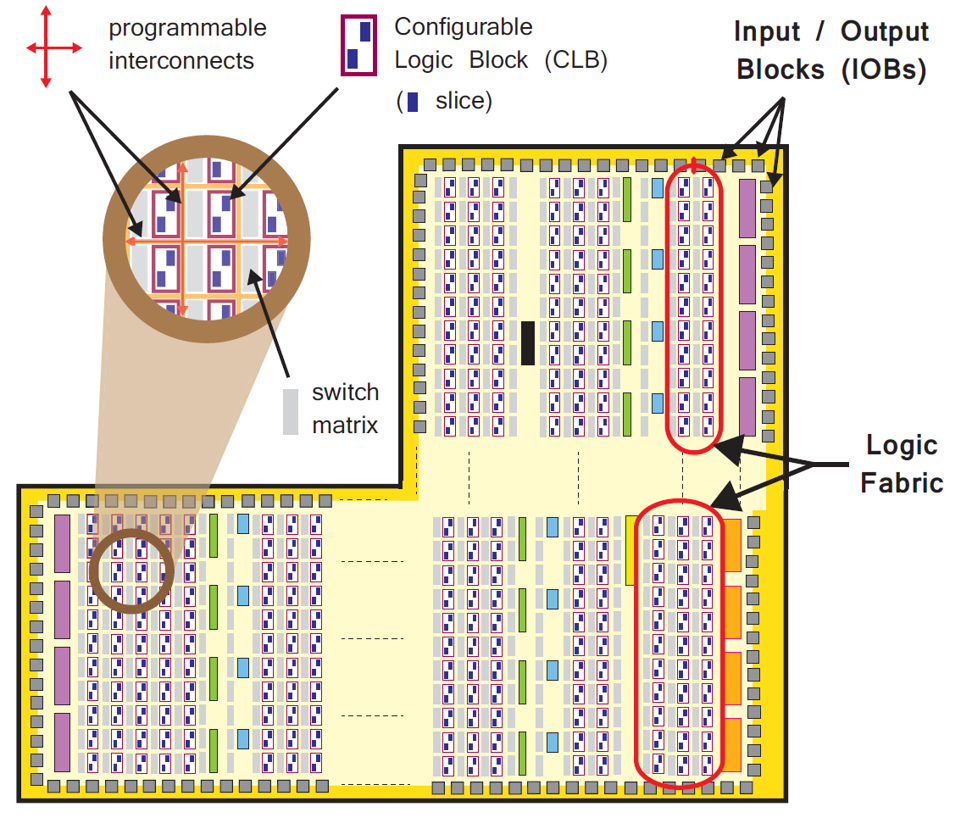
\includegraphics[width=0.5\textwidth]{images/Aufbau_PL.png}
    \end{figure}
    \ \\
\end{multicols}

\begin{multicols}{2}
    \subsection{Design Herausforderungen und Bedarf}
    \subsubsection{Herausforderungen}
    \begin{compactitem}
        \item Komplexität: Hohe Parallelität auf versch. Ebenen
        \item Heterogenität: Tools / Komponenten / Hersteller / Hardwarebeschreibung / Programmiersprache
        \item Time to market: Marktdruck
    \end{compactitem}
    \subsubsection{Bedarf}
    \begin{compactitem}
        \item Wiederverwendbarkeit: Systemfunktionalität kann nicht länger von Anfang an entwickelt werden $\rightarrow$ Komponenten und Subsysteme wiederverwenden $\rightarrow$ IP-basiertes Design
        \item Hierarchie: Weitere Hierarchiestufen sind erforderlich (sowohl Hard- wie auch Software) $\rightarrow$ IP-basiertes Design
        \item Parallel statt sequentiell: Hard- und Software sind parallel zu entwickeln
        \item Teams und Tools: Entwerfen von Systemen fordert grosse Teams und gute Werkzeuge, die die Komplexität verwalten können
    \end{compactitem}

    \ \\ \ \\
\end{multicols}

\begin{multicols}{2}
    \subsection{Traditioneller Design Flow}
     \begin{figure}[H]
     	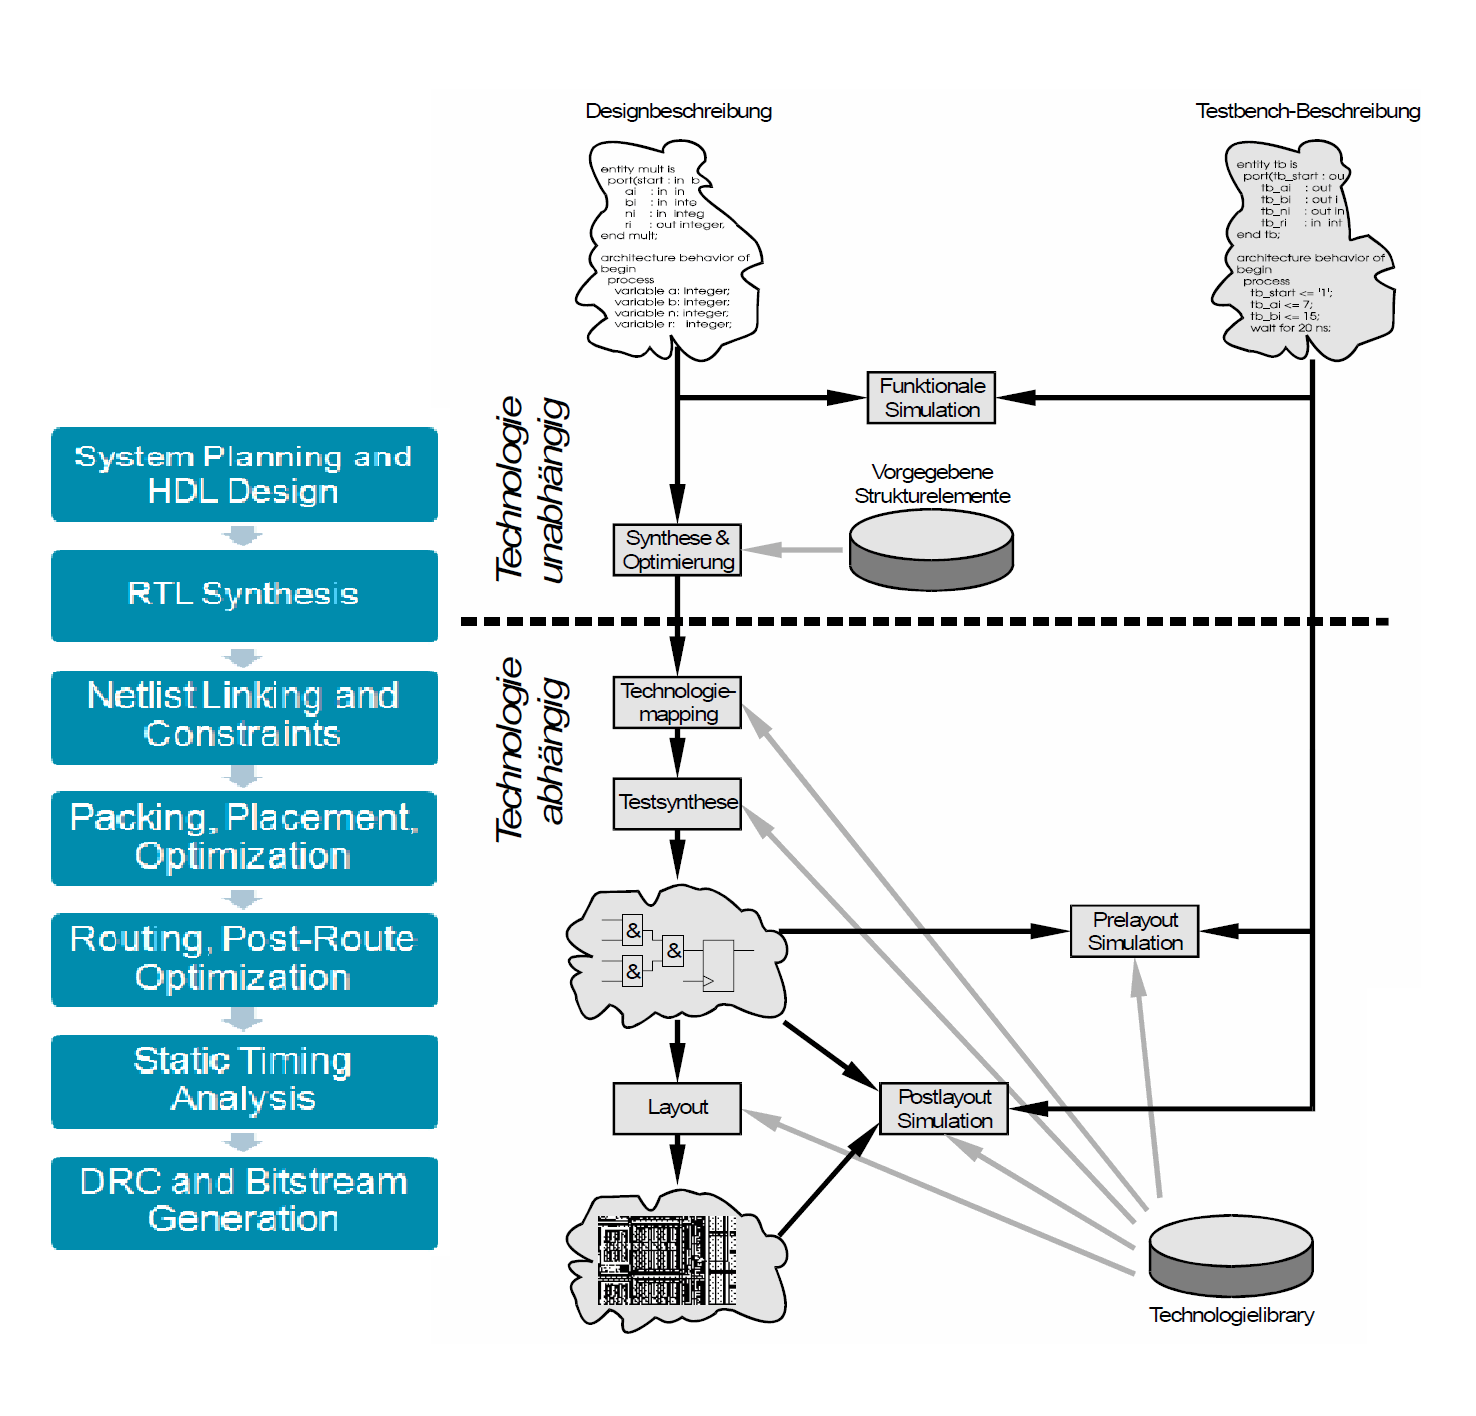
\includegraphics[width=0.53\textwidth]{images/Design_Flow_traditionell.png}
     \end{figure}
     \ \\ \ \\
    \subsection{System Level Design Flow}
    \begin{compactitem}
        \item Höhere Abstraktionsebene
        \item Partitionierung der SW und HW und Schnittstellendefinition
        \item SW/HW Co-Design
        \item System Integration $\rightarrow$ wird häufig unterschätzt
    \end{compactitem}
    \begin{figure}[H]
     	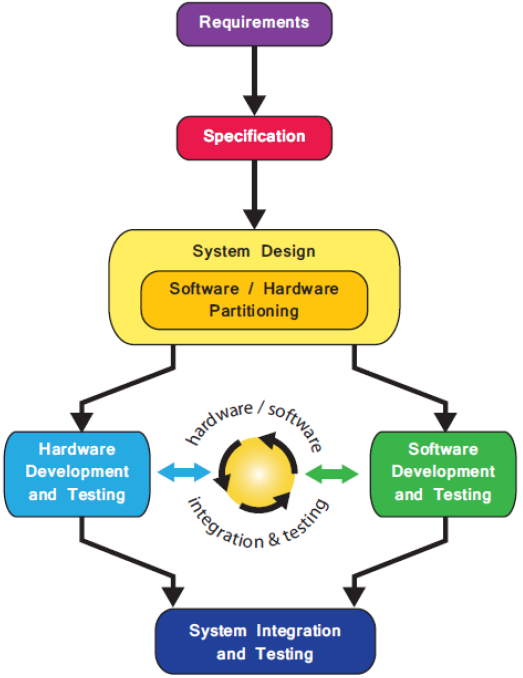
\includegraphics[width=0.35\textwidth]{images/Design_Flow_System_Level.png}
     \end{figure}
\end{multicols}
 \subsection{Design Tools}
 \subsubsection{Vivado IDE Solution}
 \paragraph{Haupteigenschaften}
 \begin{compactitem}
     \item Interaktives Design und Analyse: Timing Analysen, Konnektivität, Ressourcen Nutzung, Timinig Constraints Analysen, ..
     \item RTL Entwicklung und Analyse: Entwicklung von HDL, Hierarchische Erweiterung, Schemaerzeugung
     \item XSIM-Simulator-Integration
     \item Synthese und Umsetzung in einem Package
     \item I/O-Pin-Planung: Interaktive regelbasierte I/O Zuordnung
 \end{compactitem}
 \begin{multicols}{2}
     \paragraph{Design Database}
     Prozesse greifen auf die darunterliegende Datenbank des Designs zu. Jeder Prozess modifiziert eine vorhandene Netzliste oder erstellt eine neue. Während des ganzen Entwurfprozesses werden verschiedene Netzlisten (Elaborated, Synthesized, Implemented) verwendet.
     \subsubsection{Xilinx Software Development Kit (XSDK)}
    XSDK ist ein separates Tool von Vivado und kann eigenständig für SW-Teams installiert werden. Es ist eine voll ausgestattete Software-Design-Umgebung.
     \begin{figure}[H]
     	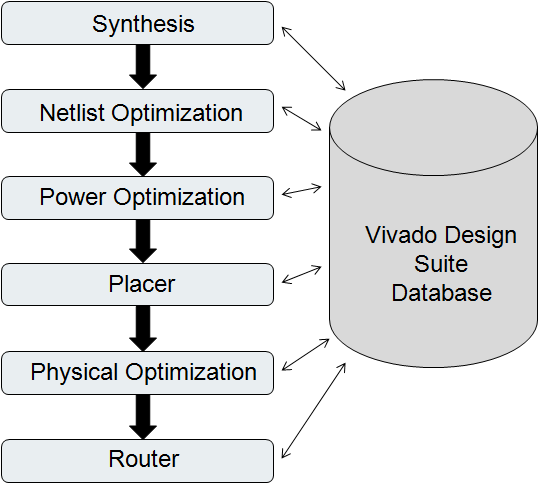
\includegraphics[width=0.25\textwidth]{images/Design_Database.png}
     \end{figure}
 \end{multicols}
